\documentclass[aspectratio=169,11pt]{beamer}

% =========================================================
% PACKAGES
% =========================================================

\usepackage[T1]{fontenc}
\usepackage{lmodern}

\usepackage{amsmath}
\usepackage{amssymb}
\usepackage{mathtools}

\usepackage{tikz}
\usetikzlibrary{positioning}

\usepackage{xcolor}
\usepackage{hyperref}

% =========================================================
% COLOURS
% =========================================================

\definecolor{MathGreen}{HTML}{446B50}
\definecolor{MathPeach}{HTML}{F7C0AA}

\definecolor{LightGreen}{HTML}{EEF3EF}
\definecolor{LightPeach}{HTML}{FDF1EC}
\definecolor{DarkText}{HTML}{222222}
\definecolor{MutedText}{HTML}{666666}

% =========================================================
% BEAMER THEME
% =========================================================

\usetheme{default}

% Remove navigation icons
\setbeamertemplate{navigation symbols}{}

% Serif typography
\usefonttheme{serif}

% =========================================================
% COLOURS
% =========================================================

\setbeamercolor{normal text}{
    fg=DarkText,
    bg=white
}

\setbeamercolor{structure}{
    fg=MathGreen
}

\setbeamercolor{frametitle}{
    fg=MathGreen,
    bg=white
}

\setbeamercolor{title}{
    fg=MathGreen
}

\setbeamercolor{subtitle}{
    fg=MutedText
}

% =========================================================
% FRAME TITLE
% =========================================================

\setbeamerfont{frametitle}{
    family=\rmfamily,
    series=\bfseries,
    size=\Large
}

\setbeamertemplate{frametitle}{
    \vspace{0.25cm}

    \begin{beamercolorbox}
        [wd=\textwidth,ht=0.65cm,dp=0.1cm]
        {frametitle}

        \usebeamerfont{frametitle}
        \insertframetitle

    \end{beamercolorbox}

    \vspace{0.05cm}

    {\color{MathPeach}\rule{\textwidth}{1.2pt}}

    \vspace{0.10cm}
}

% =========================================================
% FOOTER
% =========================================================

\setbeamertemplate{footline}{
    \leavevmode

    \hbox{
        \begin{beamercolorbox}
            [wd=.85\paperwidth,
             ht=0.38cm,
             dp=0.12cm]
            {}

            \hspace{0.7cm}

            \scriptsize
            \color{MutedText}
            Discrete Mathematics
        \end{beamercolorbox}

        \begin{beamercolorbox}
            [wd=.15\paperwidth,
             ht=0.38cm,
             dp=0.12cm]
            {}

            \scriptsize
            \color{MathGreen}
            \hfill
            \insertframenumber
            \hspace{0.7cm}
        \end{beamercolorbox}
    }
}

% =========================================================
% LISTS
% =========================================================

\setbeamertemplate{itemize item}{
    \color{MathGreen}
    $\blacktriangleright$
}

\setbeamertemplate{enumerate item}{
    \color{MathGreen}
    \insertenumlabel.
}

% =========================================================
% BLOCKS
% =========================================================

\setbeamercolor{block title}{
    fg=white,
    bg=MathGreen
}

\setbeamercolor{block body}{
    fg=DarkText,
    bg=LightGreen
}

\setbeamercolor{exampleblock title}{
    fg=DarkText,
    bg=MathPeach
}

\setbeamercolor{exampleblock body}{
    fg=DarkText,
    bg=LightPeach
}

\setbeamerfont{block title}{
    family=\rmfamily,
    series=\bfseries
}

\setbeamerfont{block body}{
    family=\rmfamily
}

% =========================================================
% SPACING
% =========================================================

\setlength{\parskip}{4pt}

\setlength{\abovedisplayskip}{6pt}
\setlength{\belowdisplayskip}{6pt}

% =========================================================
% HYPERLINKS
% =========================================================

\hypersetup{
    colorlinks=true,
    urlcolor=MathGreen,
    linkcolor=MathGreen
}

% =========================================================
% TITLE INFORMATION
% =========================================================

\title{Set Theory}

\subtitle{
    Sets, Operations, Counting and Order
}

\author{
    \textbf{Fathime Rida PS}
}

\institute{
    \textbf{Cochin University of Science and Technology (CUSAT)}
    \\[0.15cm]
    5th Semester IMSC CS (DS \& AI)
}

\date{}
% =========================================================
% DOCUMENT
% =========================================================

\begin{document}

% =========================================================
% TITLE SLIDE
% =========================================================

\begin{frame}[plain]

\vspace{0.55cm}

\begin{center}

{\Large
\color{MathGreen}
\textsc{Discrete Mathematics}
}

\vspace{0.35cm}

{\Huge
\bfseries
Introduction To Set Theory
}

\vspace{0.25cm}

{\color{MathPeach}
\rule{0.35\textwidth}{1.5pt}
}

\vspace{0.3cm}

{\large
Sets, Operations, Counting and Order
}

\end{center}

\vfill

% ---------------------------------------------------------
% Student information
% ---------------------------------------------------------

\begin{flushleft}

\color{MathGreen}
\textbf{Fathime Rida PS}

\vspace{0.08cm}

\color{DarkText}
Cochin University of Science and Technology (CUSAT)

\vspace{0.05cm}

IMSc. Computer Science (DS \& AI)

\end{flushleft}

\vspace{0.25cm}

\end{frame}

% =========================================================
% CONTENTS
% =========================================================

\begin{frame}{Contents}

\begin{enumerate}

\item Sets

\vspace{0.12cm}

\item Set Builder Form

\vspace{0.12cm}

\item Types of Sets

\vspace{0.12cm}

\item Set Operations

\vspace{0.12cm}

\item Inclusion--Exclusion Principle

\vspace{0.12cm}

\item Hasse Diagrams

\end{enumerate}

\end{frame}

% =========================================================
% SECTION 1
% =========================================================

\section{Sets}

% ---------------------------------------------------------

\begin{frame}{What is a Set?}

\begin{block}{Definition}

A \textbf{set} is a well-defined collection of objects.

\end{block}

\vspace{0.35cm}

The objects belonging to a set are called its \textcolor{MathGreen}{elements}
or \textcolor{MathGreen}{members}.

\end{frame}

% ---------------------------------------------------------

\begin{frame}{Notation for Sets}

Sets are usually denoted by capital letters:

\[
A,\qquad B,\qquad C.
\]

\vspace{0.3cm}

Elements are enclosed in braces:

\[
A=\{1,2,3,4\}.
\]

\vspace{0.3cm}

Thus,

\[
1,2,3,4\in A.
\]

\end{frame}

% ---------------------------------------------------------

\begin{frame}{Membership}

If $x$ is an element of $A$, we write

\[
\boxed{x\in A}.
\]

\vspace{0.3cm}

If $x$ is not an element of $A$, we write

\[
\boxed{x\notin A}.
\]

\vspace{0.35cm}

\begin{exampleblock}{Example}

If

\[
A=\{2,4,6,8\},
\]

then

\[
4\in A,
\qquad
5\notin A.
\]

\end{exampleblock}

\end{frame}

% ---------------------------------------------------------

\begin{frame}{Equality of Sets}

Two sets are equal when they contain exactly the same
elements.

\[
\boxed{A=B}
\]

if and only if

\[
\boxed{
\forall x\;(x\in A\iff x\in B)
}.
\]

\vspace{0.35cm}

For example,

\[
\{1,2,3\}=\{3,1,2\}.
\]

\end{frame}

% ---------------------------------------------------------

\begin{frame}{Order and Repetition}

The order of elements does not matter.

\[
\{1,2,3\}
=
\{3,2,1\}.
\]

\vspace{0.3cm}

Repeated elements are also ignored.

\[
\{1,1,2,2,3\}
=
\{1,2,3\}.
\]

\vspace{0.35cm}

A set records \textcolor{MathGreen}{membership}, not order or repetition.

\end{frame}

% ---------------------------------------------------------

\begin{frame}{Cardinality}

The number of elements in a finite set is called its
\textcolor{MathGreen}{cardinality}.

It is denoted by

\[
|A|.
\]

\vspace{0.35cm}

If

\[
A=\{2,4,6,8\},
\]

then

\[
\boxed{|A|=4}.
\]

\end{frame}

% =========================================================
% SECTION 2
% =========================================================

\section{Set Builder Form}

% ---------------------------------------------------------

\begin{frame}{Set Builder Form}

A set can be described by stating a condition that its
elements satisfy.

\vspace{0.35cm}

The general form is

\[
\boxed{
A=\{x\in U\mid P(x)\}
}
\]

where $P(x)$ is a condition on $x$.

\end{frame}

% ---------------------------------------------------------

\begin{frame}{Reading Set Builder Form}

Consider

\[
A=\{x\in\mathbb N\mid x<6\}.
\]

\vspace{0.4cm}

This means:

\begin{center}

\textit{The set of all natural numbers $x$ such that $x<6$.}

\end{center}

\vspace{0.4cm}


\end{frame}

% ---------------------------------------------------------

\begin{frame}{Example: Natural Numbers}

Consider

\[
A=\{x\in\mathbb N\mid x<6\}.
\]

\vspace{0.35cm}

In roster form,

\[
\boxed{
A=\{1,2,3,4,5\}.
}
\]

\vspace{0.35cm}

The two forms describe the same set.

\end{frame}

% ---------------------------------------------------------

\begin{frame}{Example: Even Numbers}

The even natural numbers less than $10$ can be written as

\[
\boxed{
A=
\{x\in\mathbb N
\mid
x<10
\text{ and }
2\mid x
\}.
}
\]

\vspace{0.4cm}

In roster form,

\[
A=\{2,4,6,8\}.
\]

\end{frame}

% =========================================================
% SECTION 3
% =========================================================

\section{Types of Sets}

% ---------------------------------------------------------

\begin{frame}{Types of Sets}

Important types of sets include:

\begin{itemize}

\item Empty set

\item Singleton set

\item Finite set

\item Infinite set

\item Subset

\item Proper subset

\item Power set

\end{itemize}

\end{frame}

% ---------------------------------------------------------

\begin{frame}{Empty Set}

\begin{block}{Definition}

The \textbf{empty set} is the set containing no elements.

\end{block}

\vspace{0.35cm}

It is denoted by

\[
\boxed{\varnothing}.
\]

\vspace{0.3cm}

For example,

\[
\{x\in\mathbb N\mid x<0\}
=
\varnothing.
\]

\end{frame}

% ---------------------------------------------------------

\begin{frame}{Singleton Set}

\begin{block}{Definition}

A \textbf{singleton set} contains exactly one element.

\end{block}

\vspace{0.35cm}

For example,

\[
A=\{7\}.
\]

Therefore,

\[
\boxed{|A|=1}.
\]

\end{frame}

% ---------------------------------------------------------

\begin{frame}{Finite and Infinite Sets}

A set is \textbf{finite} if it contains a finite number
of elements.

\[
A=\{1,2,3,4,5\}.
\]

\vspace{0.35cm}

A set is \textbf{infinite} if it is not finite.

\[
\mathbb N=\{1,2,3,\ldots\}.
\]

\end{frame}

% ---------------------------------------------------------

\begin{frame}{Subset}

\begin{block}{Definition}

$A$ is a subset of $B$ if every element of $A$ is also
an element of $B$.

\end{block}

\vspace{0.35cm}

We write

\[
\boxed{A\subseteq B}.
\]

\vspace{0.3cm}

Equivalently,

\[
A\subseteq B
\iff
\forall x\,(x\in A\Rightarrow x\in B).
\]

\end{frame}

% ---------------------------------------------------------

\begin{frame}{Subset: Example}

Let

\[
A=\{1,2\}
\]

and

\[
B=\{1,2,3,4\}.
\]

\vspace{0.35cm}

Since every element of $A$ belongs to $B$,

\[
\boxed{A\subseteq B}.
\]

\end{frame}

% ---------------------------------------------------------

\begin{frame}{Proper Subset}

If

\[
A\subseteq B
\]

and

\[
A\neq B,
\]

then $A$ is called a \textcolor{MathGreen}{proper subset} of $B$.

\vspace{0.35cm}

We write

\[
\boxed{A\subset B}.
\]

\end{frame}

% ---------------------------------------------------------

\begin{frame}{Power Set}

\begin{block}{Definition}

The \textbf{power set} of $A$, denoted by $\mathcal P(A)$,
is the set of all subsets of $A$.

\end{block}

\vspace{0.3cm}

For

\[
A=\{a,b\},
\]

we have

\[
\mathcal P(A)
=
\{
\varnothing,
\{a\},
\{b\},
\{a,b\}
\}.
\]

\end{frame}

% ---------------------------------------------------------

\begin{frame}{Cardinality of a Power Set}

If

\[
|A|=n,
\]

then

\[
\boxed{
|\mathcal P(A)|=2^n.
}
\]

\vspace{0.35cm}

For example, if

\[
|A|=3,
\]

then

\[
|\mathcal P(A)|=2^3=8.
\]

\end{frame}

% =========================================================
% SECTION 4
% =========================================================

\section{Set Operations}

% ---------------------------------------------------------

\begin{frame}{Set Operations}

The fundamental operations are:

\begin{center}

\[
A\cup B
\qquad
A\cap B
\qquad
A-B
\qquad
A^c
\]

\end{center}

\vspace{0.35cm}

They allow us to construct new sets from existing sets.

\end{frame}

% ---------------------------------------------------------

\begin{frame}{Union}

\begin{block}{Definition}

The union of $A$ and $B$ consists of all elements that
belong to $A$ or to $B$.

\end{block}

\vspace{0.35cm}

It is written

\[
\boxed{A\cup B}.
\]

\vspace{0.3cm}

\[
x\in A\cup B
\iff
(x\in A)\lor(x\in B).
\]

\end{frame}

% ---------------------------------------------------------

\begin{frame}{Union: Example}

Let

\[
A=\{1,2,3\}
\]

and

\[
B=\{3,4,5\}.
\]

Then

\[
\boxed{
A\cup B=\{1,2,3,4,5\}.
}
\]

\vspace{0.3cm}

The common element $3$ appears only once.

\end{frame}

% ---------------------------------------------------------

\begin{frame}{Intersection}

\begin{block}{Definition}

The intersection of $A$ and $B$ consists of the elements
common to both sets.

\end{block}

\vspace{0.35cm}

It is written

\[
\boxed{A\cap B}.
\]

\vspace{0.3cm}

\[
x\in A\cap B
\iff
(x\in A)\land(x\in B).
\]

\end{frame}

% ---------------------------------------------------------

\begin{frame}{Intersection: Example}

Let

\[
A=\{1,2,3\}
\]

and

\[
B=\{3,4,5\}.
\]

Then

\[
\boxed{
A\cap B=\{3\}.
}
\]

\vspace{0.35cm}

The intersection contains only the common elements.

\end{frame}

% ---------------------------------------------------------

\begin{frame}{Set Difference}

\begin{block}{Definition}

The difference $A-B$ consists of the elements that belong
to $A$ but do not belong to $B$.

\end{block}

\vspace{0.35cm}

\[
\boxed{
A-B=\{x\mid x\in A,\ x\notin B\}.
}
\]

\end{frame}

% ---------------------------------------------------------

\begin{frame}{Difference: Example}

Let

\[
A=\{1,2,3,4\}
\]

and

\[
B=\{3,4,5,6\}.
\]

Then

\[
\boxed{
A-B=\{1,2\}.
}
\]

\[
\boxed{
B-A=\{5,6\}.
}
\]

\end{frame}

% ---------------------------------------------------------

\begin{frame}{Complement}

Let $U$ be the universal set.

\begin{block}{Definition}

The complement of $A$ consists of all elements of $U$
that do not belong to $A$.

\end{block}

\vspace{0.35cm}

It is written

\[
\boxed{A^c}.
\]

\end{frame}

% ---------------------------------------------------------

\begin{frame}{Complement: Example}

Let

\[
U=\{1,2,3,4,5,6\}
\]

and

\[
A=\{1,2,3\}.
\]

Then

\[
\boxed{
A^c=\{4,5,6\}.
}
\]

\end{frame}

% ---------------------------------------------------------

\begin{frame}{De Morgan's Laws}

Two important identities are

\[
\boxed{
(A\cup B)^c=A^c\cap B^c
}
\]

and

\[
\boxed{
(A\cap B)^c=A^c\cup B^c.
}
\]

\vspace{0.4cm}

These laws connect complements with union and intersection.

\end{frame}

% =========================================================
% SECTION 5
% =========================================================

\section{Inclusion--Exclusion Principle}

% ---------------------------------------------------------

\begin{frame}{The Counting Problem}

Suppose we want to find

\[
|A\cup B|.
\]

A first attempt might be

\[
|A|+|B|.
\]

\vspace{0.35cm}

But elements in

\[
A\cap B
\]

have been counted twice.

\end{frame}

% ---------------------------------------------------------

\begin{frame}{The Inclusion--Exclusion Principle}

We subtract the overlap once.

\[
\boxed{
|A\cup B|
=
|A|+|B|-|A\cap B|.
}
\]

\vspace{0.45cm}

The formula corrects the double counting.

\end{frame}

% ---------------------------------------------------------

\begin{frame}{Example}

Suppose

\[
|A|=30,
\qquad
|B|=25,
\qquad
|A\cap B|=10.
\]

Then

\[
|A\cup B|
=
30+25-10.
\]

Therefore,

\[
\boxed{
|A\cup B|=45.
}
\]

\end{frame}

% ---------------------------------------------------------

\begin{frame}{Three Sets}

For three sets,

\[
A,\quad B,\quad C,
\]

we have

\[
\boxed{
\begin{aligned}
|A\cup B\cup C|
={}&|A|+|B|+|C|\\
&-|A\cap B|-|B\cap C|-|C\cap A|\\
&+|A\cap B\cap C|.
\end{aligned}
}
\]

\end{frame}

% =========================================================
% SECTION 6
% =========================================================

\section{Hasse Diagrams}

% ---------------------------------------------------------

\begin{frame}{Partially Ordered Sets}

A \textcolor{MathGreen}{partial order} is a relation satisfying:

\begin{itemize}

\item Reflexivity

\item Antisymmetry

\item Transitivity

\end{itemize}

\vspace{0.25cm}

A set together with a partial order is called a

\begin{center}

\Large
\textcolor{MathGreen}{\textbf{partially ordered set}}
\end{center}

or \textcolor{MathGreen}{poset}.

\end{frame}

% ---------------------------------------------------------

\begin{frame}{Hasse Diagrams}

A Hasse diagram is a graphical representation of a
partially ordered set.

\vspace{0.35cm}

It emphasizes the essential ordering relationships.

\vspace{0.35cm}

Relations that can be inferred through transitivity
are not drawn.

\end{frame}

% ---------------------------------------------------------

\begin{frame}{Cover Relation}

Suppose

\[
a<b.
\]

If there is no element $c$ such that

\[
a<c<b,
\]

then $b$ \textbf{covers} $a$.

\vspace{0.35cm}

A line is drawn between $a$ and $b$.

\end{frame}

% ---------------------------------------------------------

\begin{frame}{Simple Hasse Diagram}

Consider

\[
\{1,2,3\}
\]

with the usual order.

\vspace{0.2cm}

\begin{center}

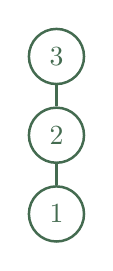
\begin{tikzpicture}[
    every node/.style={
        circle,
        draw=MathGreen,
        line width=0.9pt,
        minimum size=0.7cm,
        text=MathGreen
    },
    every path/.style={
        draw=MathGreen,
        line width=0.9pt
    }
]

\node (3) at (0,2) {$3$};
\node (2) at (0,1) {$2$};
\node (1) at (0,0) {$1$};

\draw (1)--(2);
\draw (2)--(3);

\end{tikzpicture}

\end{center}

\end{frame}

% ---------------------------------------------------------

\begin{frame}{Hasse Diagram and Divisibility}

Consider

\[
S=\{1,2,3,6\}
\]

with the relation

\[
a\mid b.
\]

\vspace{0.3cm}

For example,

\[
1\mid2,
\qquad
1\mid3,
\qquad
2\mid6,
\qquad
3\mid6.
\]

\end{frame}

% ---------------------------------------------------------

\begin{frame}{Divisibility Hasse Diagram}

\begin{center}

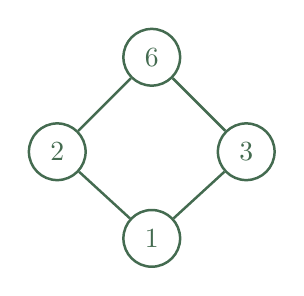
\begin{tikzpicture}[
    every node/.style={
        circle,
        draw=MathGreen,
        line width=0.9pt,
        minimum size=0.72cm,
        text=MathGreen
    },
    every path/.style={
        draw=MathGreen,
        line width=0.9pt
    }
]

\node (6) at (0,2.3) {$6$};

\node (2) at (-1.2,1.1) {$2$};
\node (3) at (1.2,1.1) {$3$};

\node (1) at (0,0) {$1$};

\draw (1)--(2);
\draw (1)--(3);
\draw (2)--(6);
\draw (3)--(6);

\end{tikzpicture}

\end{center}

\end{frame}

% ---------------------------------------------------------

\begin{frame}{Power Set as a Poset}

Consider

\[
A=\{a,b\}.
\]

Its power set is

\[
\mathcal P(A)
=
\{
\varnothing,
\{a\},
\{b\},
\{a,b\}
\}.
\]

\vspace{0.3cm}

Order these sets using

\[
\subseteq.
\]

\end{frame}

% ---------------------------------------------------------

\begin{frame}{Hasse Diagram of $\mathcal P(\{a,b\})$}

\begin{center}

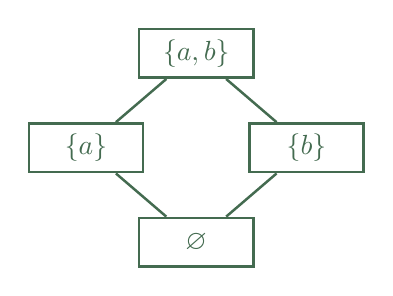
\begin{tikzpicture}[
    every node/.style={
        draw=MathGreen,
        line width=0.9pt,
        minimum width=1.45cm,
        minimum height=0.62cm,
        text=MathGreen
    },
    every path/.style={
        draw=MathGreen,
        line width=0.9pt
    }
]

\node (top) at (0,2.4) {$\{a,b\}$};

\node (a) at (-1.4,1.2) {$\{a\}$};
\node (b) at (1.4,1.2) {$\{b\}$};

\node (empty) at (0,0) {$\varnothing$};

\draw (empty)--(a);
\draw (empty)--(b);

\draw (a)--(top);
\draw (b)--(top);

\end{tikzpicture}

\end{center}

\vspace{0.2cm}

\begin{center}

\textcolor{MutedText}
{
The ordering relation is $\subseteq$.
}

\end{center}

\end{frame}

% =========================================================
% SUMMARY
% =========================================================

\section{Summary}

% ---------------------------------------------------------

\begin{frame}{Summary}

\begin{itemize}

\item A set is a well-defined collection of objects.

\vspace{0.12cm}

\item Set-builder notation describes sets using conditions.

\vspace{0.12cm}

\item Sets may be empty, finite, infinite, or related by
subsets.

\vspace{0.12cm}

\item Union, intersection, difference and complement are
fundamental set operations.

\vspace{0.12cm}

\item Inclusion--exclusion provides a method for correcting
double counting.

\vspace{0.12cm}

\item Hasse diagrams represent partially ordered sets
visually.

\end{itemize}

\end{frame}

% =========================================================
% FORMULAS
% =========================================================

\begin{frame}{Important Formulas}

\begin{center}

\[
\boxed{
|A\cup B|
=
|A|+|B|-|A\cap B|
}
\]

\vspace{0.18cm}

\[
\boxed{
|\mathcal P(A)|=2^{|A|}
}
\]

\vspace{0.18cm}

\[
\boxed{
(A\cup B)^c=A^c\cap B^c
}
\]

\vspace{0.18cm}

\[
\boxed{
(A\cap B)^c=A^c\cup B^c
}
\]

\end{center}

\end{frame}

% =========================================================
% REFERENCE
% =========================================================

\begin{frame}{Reference}

\begin{block}{Primary Reference}

Stanford Encyclopedia of Philosophy

\vspace{0.15cm}

\textit{Set Theory}

\vspace{0.15cm}

\url{https://plato.stanford.edu/entries/set-theory/}

\end{block}

\vspace{0.4cm}

The presentation uses the reference for the foundational
treatment of sets, membership, subsets, set operations and
related concepts.

\end{frame}

% =========================================================
% FINAL SLIDE
% =========================================================

\begin{frame}[plain]

\vspace{1.5cm}

\begin{center}

{\Huge
\color{MathGreen}
\textsc{Thank You}
}

\vspace{0.4cm}

{\color{MathPeach}
\rule{0.28\textwidth}{1.5pt}
}

\vspace{0.4cm}

\end{center}

\end{frame}

% =========================================================

\end{document}
